\begin{frame}<2>[noframenumbering,fragile,label=cpuAndMemory]{processors and memory}
\begin{tikzpicture}
\tikzset{
    box/.style={draw,rectangle,minimum width=3cm, minimum height=3cm},
    smallBox/.style={draw,rectangle,minimum width=2cm, minimum height=2cm},
    bigBox/.style={draw,rectangle,minimum width=5cm, minimum height=5cm},
}
\node[anchor=center] (cpu)  {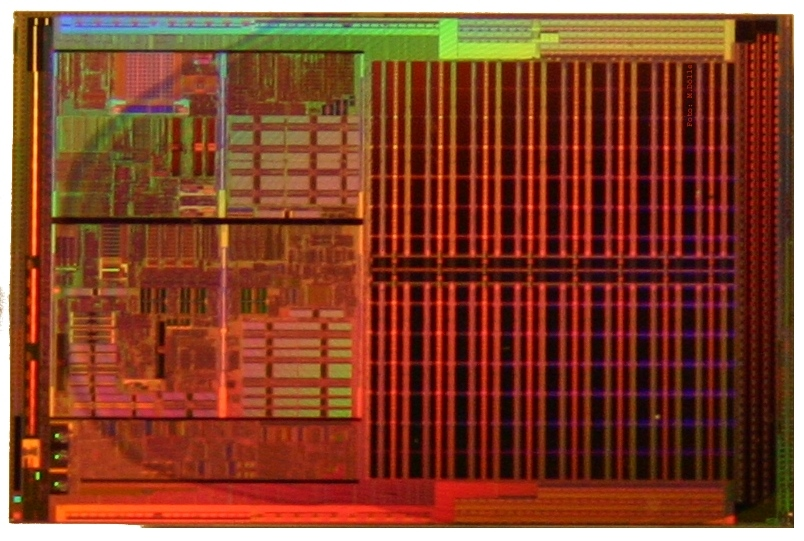
\includegraphics[width=3cm]{Opteron-die.jpg}};
\node[below=-2pt of cpu] {processor};
\node[anchor=center,right=8cm of cpu] (memory) {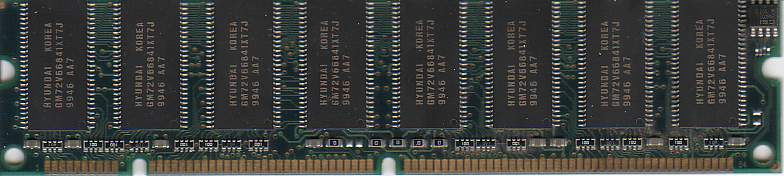
\includegraphics[height=0.75cm,angle=90]{SDRAM.jpg}};
\node[below=0pt of memory] {memory};

\onslide<1-3|handout:0>{
    \draw[latex-latex, line width=3pt] (cpu) -- (memory);
}
\coordinate (middleBus) at ($(cpu)!.5!(memory)$);


\onslide<3|handout:0>{
    \node[my callout2=middleBus,align=left] at ($(middleBus) + (-3cm,2cm)$) {memory bus \\ send address + send or get data};
}

\onslide<4->{
    \node[smallBox,anchor=center,fill=white, align=center] (ioBridge) at (middleBus) {I/O \\ Bridge};
    \draw[latex-latex, line width=3pt] (cpu) -- (ioBridge);
    \draw[latex-latex, line width=3pt] (ioBridge) -- (memory);
    \coordinate (toIO) at ($(middleBus) + (0,-3cm)$);
    \draw[latex-latex, line width=3pt] (ioBridge) -- (toIO);
    \node[below=0pt of toIO, align=left] {to I/O devices \\ \small keyboard, mouse, wifi, \ldots};
    \coordinate (middleSysBus) at ($(cpu)!.5!(middleBus)$);
    \coordinate (middleMemBus) at ($(memory)!.5!(middleBus)$);
    \coordinate (middleIOBus) at ($(middleBus)!.5!(toIO)$);
}
\onslide<5>{
    \node[my callout2=middleSysBus,align=left] at ($(middleSysBus) + (0,2cm)$) {system bus \\ send address + send or get data \\ (machine code/text/number\ldots)};
}
\onslide<6-7>{
    \node[my callout2=middleSysBus,align=left] at ($(middleSysBus) + (0,2cm)$) {CPU: send PC: {\tt 0x04000}};
    \node[my callout2=middleMemBus,align=left] at ($(middleMemBus) + (-3cm,-2cm)$) {MEM: send machine code:\\{\tt pushq \%rbp}};
}
\onslide<7>{
    \node[my callout2=middleSysBus,align=left] at ($(middleSysBus) + (0,1cm)$) {CPU: next PC: {\tt 0x04001}};
}
\onslide<8>{
    \node[my callout2=middleSysBus,align=left] at ($(middleSysBus) + (-2,2cm)$) {CPU: send I/O request address: {\tt 0xf122003}};
    \node[my callout2=middleIOBus,align=left] at ($(middleIOBus) + (1cm,0)$) {I/O: send keystoke: ``a''};
}
\end{tikzpicture}
\imagecredit{Images: \\
             Single core Opteron 8xx die: Dg2fer at the German language Wikipedia, via Wikimedia Commons \\
             SDRAM by Arnaud 25, via Wikimedia Commons}
\end{frame}
